\subsection{The CML Metamodel (Abstract Syntax)}\label{subsec:metamodel}

In the article \emph{UML and OCL in Conceptual Modeling},
Gogolla \cite{gogolla} shows, by mapping the UML \cite{uml} metamodel to the ER \cite{er} metamodel,
how UML models (augmented by OCL \cite{ocl} constraints) can be used to specify conceptual models.
Also, Wazlawick \cite{wazlawick} systematically prescribes a method for conceptual modeling using UML and OCL.
Since one key CML goal is enabling the specification of conceptual models
(such as those specified by ER models and UML/OCL models),
in order to present the key elements of the CML metamodel,
a similar approach to Gogolla's is used to map the CML metamodel to the ER metamodel,
and to the UML/OCL metamodel.

The EMOF \cite{mof} model presented by figure \ref{fig:metamodel} is a simplified version of the CML metamodel.
As shown, a \emph{Concept} is composed of zero-or-more \emph{Property} instances.
Each \emph{Property} must have a \emph{Type} and an optional \emph{Expression}.
If two \emph{Property} instances represent both ends of the same bidirectional association,
there must be an \emph{Association} instance that binds them.
Unidirectional associations are only represented by a single \emph{Property} instance
(actually representing the association role)
that enables the navigation from the source \emph{Concept} instance to the target one,
which is represented by the property's \emph{Type}.

\begin{figure}
\centering
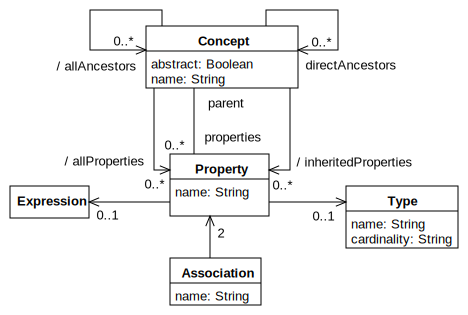
\includegraphics[width=0.8\textwidth]{language/diagram-metamodel}
\caption{Simplified EMOF \cite{mof} model defining the CML metamodel.}
\label{fig:metamodel}
\end{figure}

Next, there is a description for the key metamodel elements:

\begin{itemize}

\item \emph{Concept}: According to Wazlawick \cite{wazlawick},
a concept represents complex information that has a coherent meaning in the domain.
They aggregate attributes and cannot be described as primitive values.
They may also be associated with other concepts.
On the ER metamodel, it is known as \emph{Entity Type};
on the UML metamodel, as \emph{Class}.
CML's \emph{Concept} differs, however, from the UML \emph{Class},
because it has only \emph{Property} instances,
while the UML \emph{Class} may also have \emph{Operation} instances.

\item \emph{Property}: May hold values of primitive types, in which case they represent an attribute on the \emph{ER} and \emph{UML} metamodels;
or may hold references (or collections of references) linking to instances of other concepts.
On the ER metamodel,
a set of all references linking one \emph{Entity Type} to another is known as a \emph{Relationship};
on the UML metamodel, it is known as a unidirectional \emph{Association}.

\item \emph{Association}: Unlike the ER and UML metamodels, in the CML metamodel,
only a bidirectional \emph{Association} is represented with the \emph{Association} class.
Using UML terminology, they bind the reference (non-primitive) properties (of the same, or of different concepts),
so that the \emph{Association} links are accessible from each participating association end.
It directly represents in the CML metamodel what normally requires additional implementation in programming languages.
It is inspired\footnote{The syntax used in CML resembles the syntax of a \emph{struct} in C \cite{clang}, while Cardoso \cite{cardoso} uses a verbose syntax. Also, unlike CML, Cardoso does \emph{not} bind properties that represent each association end; instead, associations -- unidirectional or bidirectional -- are declared independently of class properties.} on the work of Cardoso \cite{cardoso}, which extends the C\# language to represent bidirectional associations; it is also inspired on the work of Balzer et. al. \cite{balzer}, which uses \emph{member interposition} to model relationships.

\item \emph{Type}: They may be of: a primitive type (such as Boolean, String, and Decimal); a reference to a \emph{Concept} instance (\emph{cardinality} equal to one); a sequence of references (\emph{cardinality} equal to zero-or-many); or optional, meaning their value may or may not have been set (also defined by the \emph{cardinality} property).
CML also supports the tuple and lambda types, which are used in expressions.

\item \emph{Inheritance}: Following the the UML \cite{uml} metamodel,
CML provides the generalization/specialization relationship.
In CML, a \emph{Concept} may be a specialization of two or more other \emph{Concept} instances.
If a \emph{Property} has been defined by more than one generalization,
CML requires it to be redefined by the specialization
in order to resolve the definition conflict.

\end{itemize}
